\documentclass[twoside,twocolumn]{article}
\usepackage[hmarginratio=1:1,top=32mm,columnsep=20pt]{geometry}
\usepackage[hang, small,labelfont=bf,up,textfont=it,up]{caption}
\usepackage{amssymb} 
\usepackage{amsmath}
\usepackage{booktabs}
\usepackage{enumitem}
\setlist[itemize]{noitemsep}
\usepackage{abstract}
\renewcommand{\abstractnamefont}{\normalfont\bfseries}
\renewcommand{\abstracttextfont}{\normalfont\small\itshape}
\usepackage{titlesec}
\renewcommand\thesection{\Roman{section}}
\renewcommand\thesubsection{\Alph{subsection}}
\renewcommand\thesubsubsection{\arabic{subsubsection}}
\titleformat{\section}[block]{\normalsize\bfseries\scshape\centering}{\thesection.}{1em}{}
\titleformat{\subsection}[block]{\normalsize\bfseries\centering}{\thesubsection.}{1em}{}
\titleformat{\subsubsection}[block]{\normalsize\centering}{\thesubsubsection.}{1em}{}
\usepackage{fancyhdr}
\pagestyle{fancy}
\fancyhead{}
\fancyhead[C]{Computational Physics Homework $\bullet$ May 2018 $\bullet$ Vol. I, No. 6}
\usepackage{titling}
\usepackage{hyperref}
\hypersetup{unicode}
\AtBeginShipoutFirst{\input{zhwinfonts.tex}}
\usepackage{bm}
\usepackage{braket}
\usepackage{CJKutf8}
\usepackage{xcolor}
\usepackage{dcolumn}
\usepackage{graphicx}
\usepackage{indentfirst}
\usepackage{listings}
\usepackage[toc, page, title, titletoc, header]{appendix}
\definecolor{grey}{rgb}{0.8,0.8,0.8}
\definecolor{darkgreen}{rgb}{0,0.3,0}
\definecolor{darkblue}{rgb}{0,0,0.3}
\def\lstbasicfont{\fontfamily{pcr}\selectfont\footnotesize}
\lstset{
	numbers=left,
	numberstyle=\small,
	showstringspaces=false,
	showspaces=false,
	tabsize=4,
	frame=single,
	basicstyle={\footnotesize\lstbasicfont},
	keywordstyle=\color{darkblue}\bfseries,
	identifierstyle=,
	commentstyle=\color{darkgreen},
	stringstyle=\color{black}
}
\lstloadlanguages{C,C++,Fortran,Java,Matlab,Mathematica,Python}
\setlength{\parindent}{2em}
\begin{document}
\begin{CJK*}{UTF8}{gkai}
%----------------------------------------------------------------------------------------
%	TITLE SECTION
%----------------------------------------------------------------------------------------

\setlength{\droptitle}{-4\baselineskip} % Move the title up
\pretitle{\begin{center}\Huge\bfseries} % Article title formatting
	\posttitle{\end{center}} % Article title closing formatting
\title{计算物理第六次作业} % Article title
\author{
	\textsc{梁旭民}\thanks{\noindent 指导老师:齐新老师} \\[1ex] % Your name
	\normalsize Cuiying Hornors College, Lanzhou University \\ % Your institution
	\normalsize \href{mailto:liangxm15@lzu.edu.cn}{liangxm15@lzu.edu.cn} % Your email address
}
\date{}
\renewcommand{\maketitlehookd}{
	\begin{abstract}
		本次作业学习了Box-Muller生成Gauss分布的方法及Gibbs采样法生成Gauss分布随机数的方法,并应用Box-Muller算法成功生成了一维Gauss分布的随机数,应用Gibbs采样法生成二维Gauss分布的随机数。
	\end{abstract}
}
\maketitle

%----------------------------------------------------------------------------------------
%	SECTION 1
%----------------------------------------------------------------------------------------

\section{Box-Muller算法生成Gauss分布随机数}
	\subsection{问题描述}
		通过使用Box-Muller算法,生成一组1维Gauss分布的随机数。
	\subsection{Box-Muller算法简介}
	Box-Muller变换[2]是一种由George Edward Pelham Box和Mervin Edgar Muller提出的伪随机数抽样方法,用于生成一对独立的 ,标准的,正态分布的(零期望,单位方差)随机数,给定一个源均匀分布的随机数。
	\subsubsection{基本形式}
	假设$U_{1}$和$U_{2}$是从单位区间(0,1)上的均匀分布中选择的独立样本。令
	\begin{equation*}
	\begin{aligned}
	&Z_{0}=R\cos(\Theta)=\sqrt{-2\ln U_{1}}\cos(2\pi U_{2})\\
	&Z_{1}=R\sin(\Theta)=\sqrt{-2\ln U_{1}}\sin(2\pi U_{2})
	\end{aligned}
	\end{equation*}
	则$Z_{0}$和$Z_{1}$是具有标准正态分布的独立随机变量。\\
	推导基于二维笛卡尔系统的性质[3],其中X和Y坐标由两个独立且正态分布的随机变量描述,$R_{2}$和$\Theta$(如上所示)的随机变量在相应的极性坐标也是独立的,可以表示为
	\begin{equation*}
	\begin{aligned}
		R^{2}&=-2\cdot \ln U_{1}\\
		\Theta&=2\pi U_{2}
	\end{aligned}
	\end{equation*}
	由于$R^{2}$是标准二元正态变量$(X,Y)$的范数的平方 ,因此它具有两个自由度的卡方分布。在两个自由度的特殊情况下,卡方分布与指数分布重合,上述$R^{2}$的等式是生成所需指数变量的简单方法。
	\subsubsection{极坐标形式}
	极地形式最初由J. Bell提出[4] ,然后由R. Knop修改[5]。虽然已经描述了几种不同版本的极坐标方法,但R. Knop的版本将在这里描述,因为它是最广泛使用的,部分原因是它包含在Numerical Recipes中。

	给定$u$和$v$ ,在闭区间$[-1,+1]$中独立且均匀分布,设$s=R^{2}=u^{2}+v^{2}$。(显然有$R=\sqrt{s}$)如果$s=0$或$s\geqslant1$ ,则忽略$u$和$v$,并尝试另一个对$(u,v)$。 由于$u$和$v$是均匀分布的,并且由于只允许单位圆内的点,因此s的值也将在开区间$(0,1)$中均匀分布。 后者可以通过计算区间$(0,1)$中$s$的累积分布函数来看出。 这是一个半径为$\sqrt{s}$圆形区域, 除以$\pi$。 由此我们发现概率密度函数在间隔$(0,1)$上具有常数值1。与此同时,角度$\theta$除以$2\pi$在区间$[0,1]$中均匀分布且与$s$无关。
	\begin{figure}[h]
		\centering
		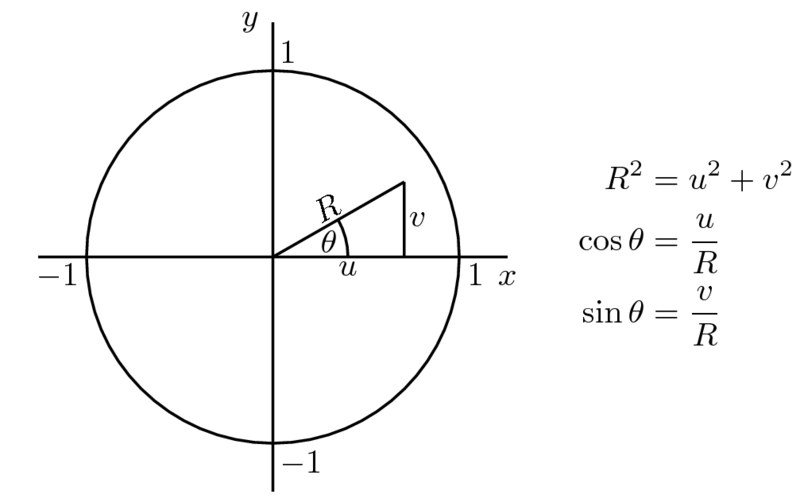
\includegraphics[width=0.7\linewidth]{figure/800px-BoxMullerTransformUsingPolarCoordinates}
		\caption{运用极坐标的Box-Muller Transform}
		\label{fig:800px-BoxMullerTransformUsingPolarCoordinates}
	\end{figure}
	我们现在确定$s$的值与$U_{1}$和的值$\frac{\theta}{2\pi}$与$U_{2}$的基本形式相同。见Figure 1,$\cos\theta=\cos(2\pi U_{2})$和$\sin\theta=\sin(2\pi U_{2})$在基本形式中的值可以用比例$\cos\theta=\frac{u}{R}=\frac{u}{\sqrt{s}}$和$\sin\theta=\frac{v}{R}=\frac{v}{\sqrt{s}}$分别代替。其优点是可以避免直接计算三角函数。 当三角函数计算成本比单个分割代替每个函数更昂贵时,这会很有帮助。
	
	正如基本形式产生两个标准正常偏差一样,这种替代计算也是如此。
	\begin{equation*}
	\begin{aligned}
	z_{0}&={\sqrt {-2\ln U_{1}}}\cos(2\pi U_{2})={\sqrt {-2\ln s}}\left({\frac {u}{\sqrt {s}}}\right)\\
	&=u\cdot {\sqrt {\frac {-2\ln s}{s}}}]\\
	z_{1}&={\sqrt {-2\ln U_{1}}}\sin(2\pi U_{2})={\sqrt {-2\ln s}}\left({\frac {v}{\sqrt {s}}}\right)\\
	&=v\cdot {\sqrt {\frac {-2\ln s}{s}}}
	\end{aligned}
	\end{equation*}
\subsubsection{标准形式和极坐标形式对比}
	极坐标法与基本方法的区别在于它是一种拒绝采样 。 它丢弃一些生成的随机数,但可以比基本方法更快,因为它计算起来更简单(假设随机数发生器相对较快)并且更具数值稳健性[6]。它避免了使用三角函数,这在一些计算环境中可能是昂贵的。 它丢弃生成的总输入均匀分布随机数对的$1-\frac{\pi}{4}\approx21.46\%$,即每生成一个高斯随机数对丢弃$\frac{4}{\pi}-1=27.32\%$均匀分布的随机数对,需要$\frac{4}{\pi}\approx1.2732$输入每个输出随机数的随机数。
	
	基本形式对于每个正态变量需要两次乘法,$\frac{1}{2}$对数,$\frac{1}{2}$平方根和一个三角函数[7]。在某些处理器上,可以使用单个指令并行计算同一个参数的余弦和正弦。 值得注意的是,对于基于Intel的机器,可以使用fsincos汇编程序指令或expi指令(通常可从C获得,作为内部函数)来计算复杂度
	\begin{equation*}
	e^{iz}=e^{iz}=\cos(z)+i\sin(z)
	\end{equation*}
	并分开实部和虚部。
	
	注:要明确计算复极点形式,请在通用形式中使用以下替换,令
	\begin{equation*}
	\begin{aligned}
	 &r={\sqrt {-2ln(u_{1})}}\\
	 &z=2\pi u_{2}
	\end{aligned}
	\end{equation*}
	则有
	\begin{equation*}
	\begin{aligned}
	re^{iz}&={\sqrt {-2ln(u_{1})}}e^{i2\pi u_{2}}\\
	&={\sqrt {-2ln(u_{1})}}\left[\cos(2\pi u_{2})+i\sin(2\pi u_{2})\right]
	\end{aligned}
	\end{equation*}
	极坐标形式需要$\frac{3}{2}$乘法,$\frac{1}{2}$对数,$\frac{1}{2}$平方根和每个正常变量的$\frac{1}{2}$除法。 其效果是用一个单独的分割和一个条件循环代替一个乘法和一个三角函数。

	应该指出的是,fsincos在现代CPU体系结构中变得非常快,这样拒绝采样方法的速度“收敛”就不再是事实。 同时,s的浮点除法和条件循环在拒绝采样算法中仍然是一个重要的开销,这在基本形式中是不存在的。 
\subsubsection{尾巴截断}
	当一台计算机被用来产生一个统一的随机变量时,它将不可避免地存在一些不准确的地方,因为对于如何接近0可以有一个较低的界限。如果该发生器使用每个输出值32位,则可以得到最小的非零数被生成的是$2^{-32}$。当$U_{1}$和$U_{2}$等于这个Box-Muller变换产生一个等于的正态随机变量$\sqrt {-2\ln(2^{-32})}\cos(2\pi 2^{-32})\approx 6.66$这意味着该算法不会产生超过均值6.66个标准差的随机变量。 这相当于一个比例$2.74 \times 10 ^ {-11}$由于截断而丢失。
\subsection{计算结果}
	未经过及经过Box-Muller生成的分布结果均见Figure 2.
\begin{figure}[h]
\centering
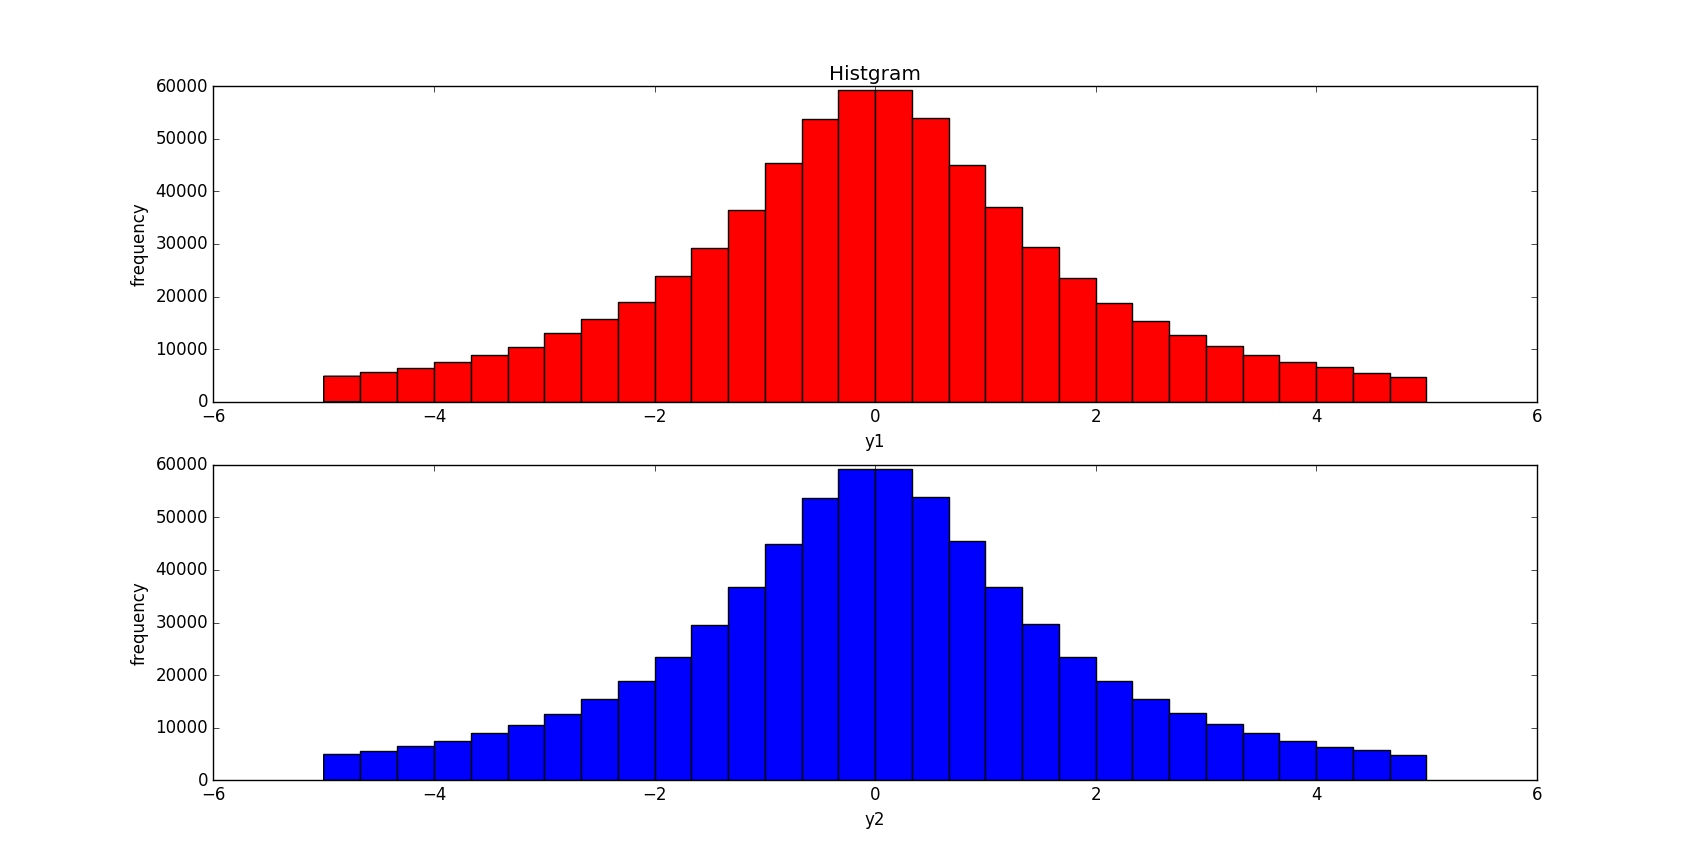
\includegraphics[width=1.0\linewidth]{figure/box-muller}
\caption{Box-Muller算法生成的一维Gauss分布}
\label{fig:box-muller}
\end{figure}
%----------------------------------------------------------------------------------------
%	SECTION 2
%----------------------------------------------------------------------------------------

\section{Gibbs采样法生成Gauss分布随机数}
	\subsection{问题描述}
		使用Gibbs采样,生成一组2维Gauss分布的随机数
	\subsection{Gibbs采样法简介}
	在统计学中 ,当直接采样困难时, Gibbs采样或Gibbs采样器是Markov chain Monte Carlo(MCMC)算法,用于获得从特定多变量概率分布近似的观察序列。 该序列可用于近似联合分布(例如,生成分布的直方图); 以近似其中一个变量的边际分布或变量的一些子集(例如未知参数或潜在变量 ); 或计算积分 (例如其中一个变量的预期值 )。 通常,一些变量对应于其值已知的观测值,因此不需要进行采样。
	
	Gibbs抽样通常被用作统计推断的手段,特别是Bayesian推断 。 它是一种随机算法 (即利用随机数的算法),是用于统计推断的确定性算法 (如期望最大化算法 (EM))的替代方法。
	
	与其他MCMC算法一样,Gibbs采样生成样本的Markov链 ,每个样本都与附近的样本相关 。 因此,如果需要独立样本,必须小心。 一般来说,从链条开始的样本( 老化期 )可能不能准确表示所需的分布,通常会被丢弃。 然而,已经表明,使用更长的链而不是更长的链(例如,使用n的稀疏因子的链是初始考虑的链的n倍)导致更好的真实后验估计。 因此,只有在限制时间或计算机内存时才应用间拔[8]。
	\subsubsection{发展简介}
	Gibbs采样是以物理学家乔西亚威拉德Gibbs的名字命名的,他提到了采样算法和统计物理学之间的类比。 该算法在1984年由Stuart和Donald Geman兄弟描述,在Gibbs死后约八十年[9]。
	
	在其基本版本中,Gibbs抽样是Metropolis-Hastings算法的特例。 然而,在其扩展版本中,它可以被认为是一个通用框架,通过对每个变量(或在某些情况下,每组变量)进行抽样,从一大组变量中抽样,并可以将Metropolis- Hastings算法 (或更复杂的方法,如切片采样 , 自适应拒绝采样和自适应拒绝Metropolis算法( [10] [11] [12] )来实现一个或多个采样步骤。
	
	Gibbs抽样适用于联合分布未明确知道或难以直接抽样的情况 ,但每个变量的条件分布是已知的并且很容易(或至少更容易)抽样。 Gibbs采样算法依次从每个变量的分布生成一个实例,取决于其他变量的当前值。 可以证明,样本序列构成一个Markov链 ,而该Markov链的平稳分布恰好是所寻求的联合分布。 [6]
	
	Gibbs采样特别适用于采样Bayesian网络的后验分布 ,因为Bayesian网络通常被指定为一组条件分布。 
	\subsubsection{算法简介}
	Gibbs抽样在其基本化身中是Metropolis-Hastings算法的特例。吉布斯采样适用于条件分布比边缘分布更容易采样的多变量分布。假设我们需要从联合分布$p(x_{1},\dots,x_{n})$中抽取$\mathbf{X} =(x_{1},\dots ,x_{n})$的$k$个样本。记第$i$个样本为$\mathbf{X} ^{(i)}=\left(x_{1}^{(i)},\dots,x_{n}^{(i)}\right)$。吉布斯采样的过程则为:
	\begin{itemize}
		\item[]{1}\quad 确定初始值 $\mathbf{X} ^{(1)}$。
		\item[]{2}\quad 假设已得到样本$\mathbf {X} ^{(i)}$,记下一个样本为$\mathbf{X} ^{(i+1)}=\left(x_{1}^{(i+1)},x_{2}^{(i+1)},\dots ,x_{n}^{(i+1)}\right)$。于是可将其看作一个向量,对其中某一分量$x_{j}^{(i+1)}$,可通过在其他分量已知的条件下该分量的概率分布来抽取该分量。对于此条件概率,我们使用样本$\mathbf {X} ^{(i+1)}$中已得到的分量$x_{1}^{(i+1)}$到$x_{j-1}^{(i+1)}$以及上一样本$\mathbf {X} ^{(i)}$中的分量$x_{j+1}^{(i)}$,即$$p\left(x_{j}^{(i+1)}|x_{1}^{(i+1)},\dots ,x_{j-1}^{(i+1)},x_{j+1}^{(i)},\dots ,x_{n}^{(i)}\right)$$
		\item[]{3}\quad 重复上述过程$k$次。
	\end{itemize}
	
	在采样完成后,我们可以用这些样本来近似所有变量的联合分布。如果仅考虑其中部分变量,则可以得到这些变量的边缘分布。此外,我们还可以对所有样本求某一变量的平均值来估计该变量的期望。
	\subsection{计算结果}
	利用Gibbs采样法产生两组不同的$\sigma$和$\mu$得到两个Gauss分布,见Figure 3.
	\begin{figure}[h]
	\centering
	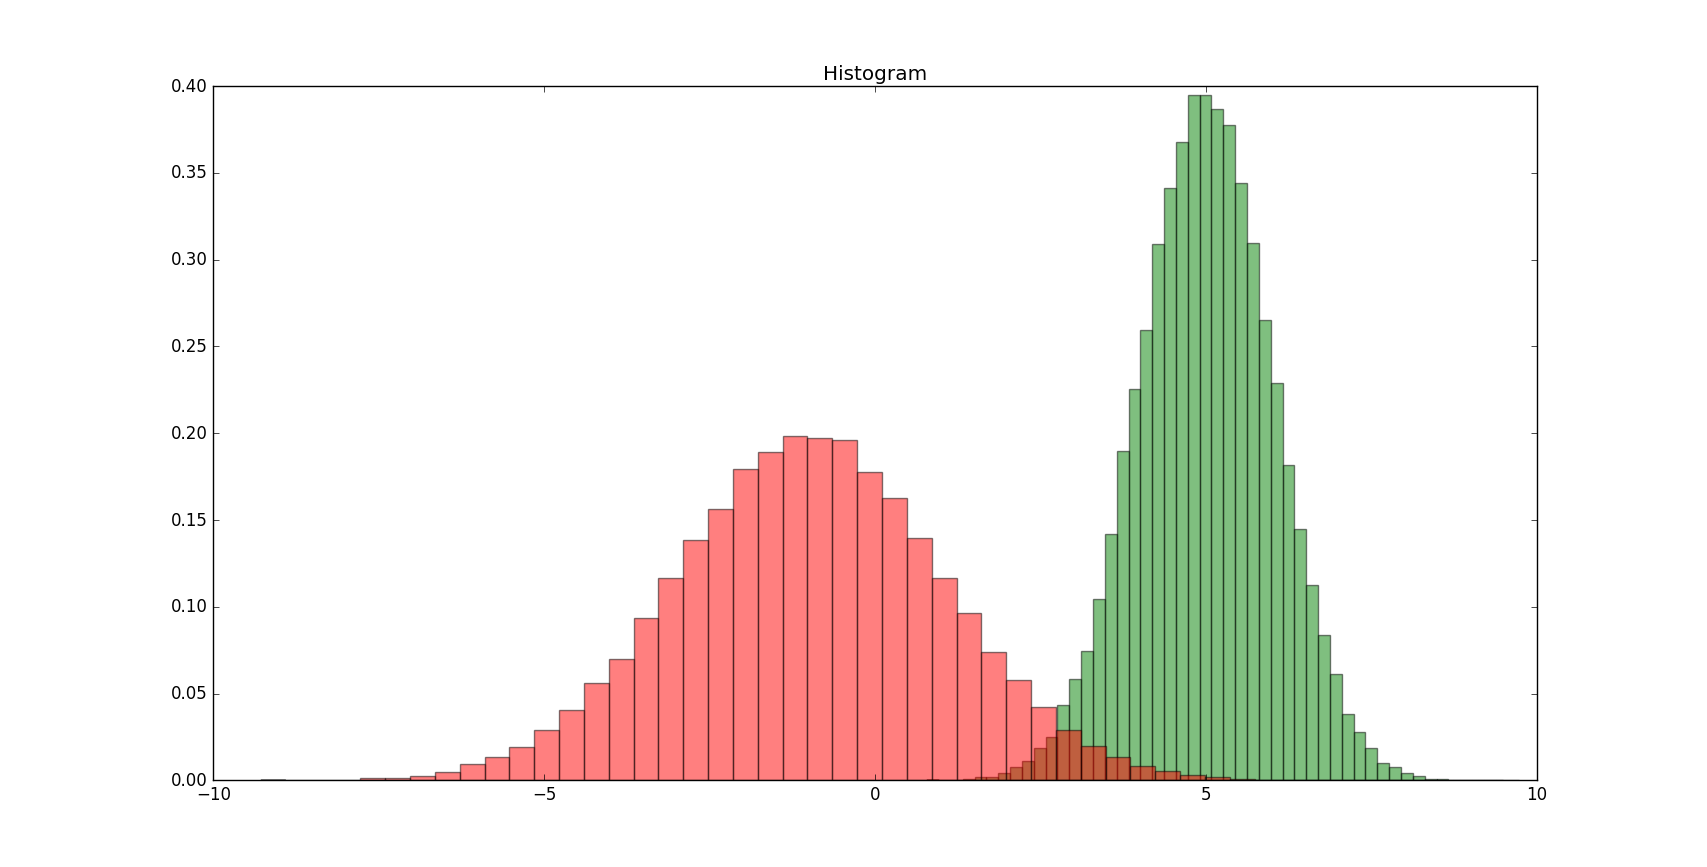
\includegraphics[width=1.0\linewidth]{figure/gibbs1}
	\caption{Gauss分布}
	\label{fig:gibbs1}
	\end{figure}
	生成的二维Gauss分布见Figure 4.
	\onecolumn
	\begin{figure}[h]
	\centering
	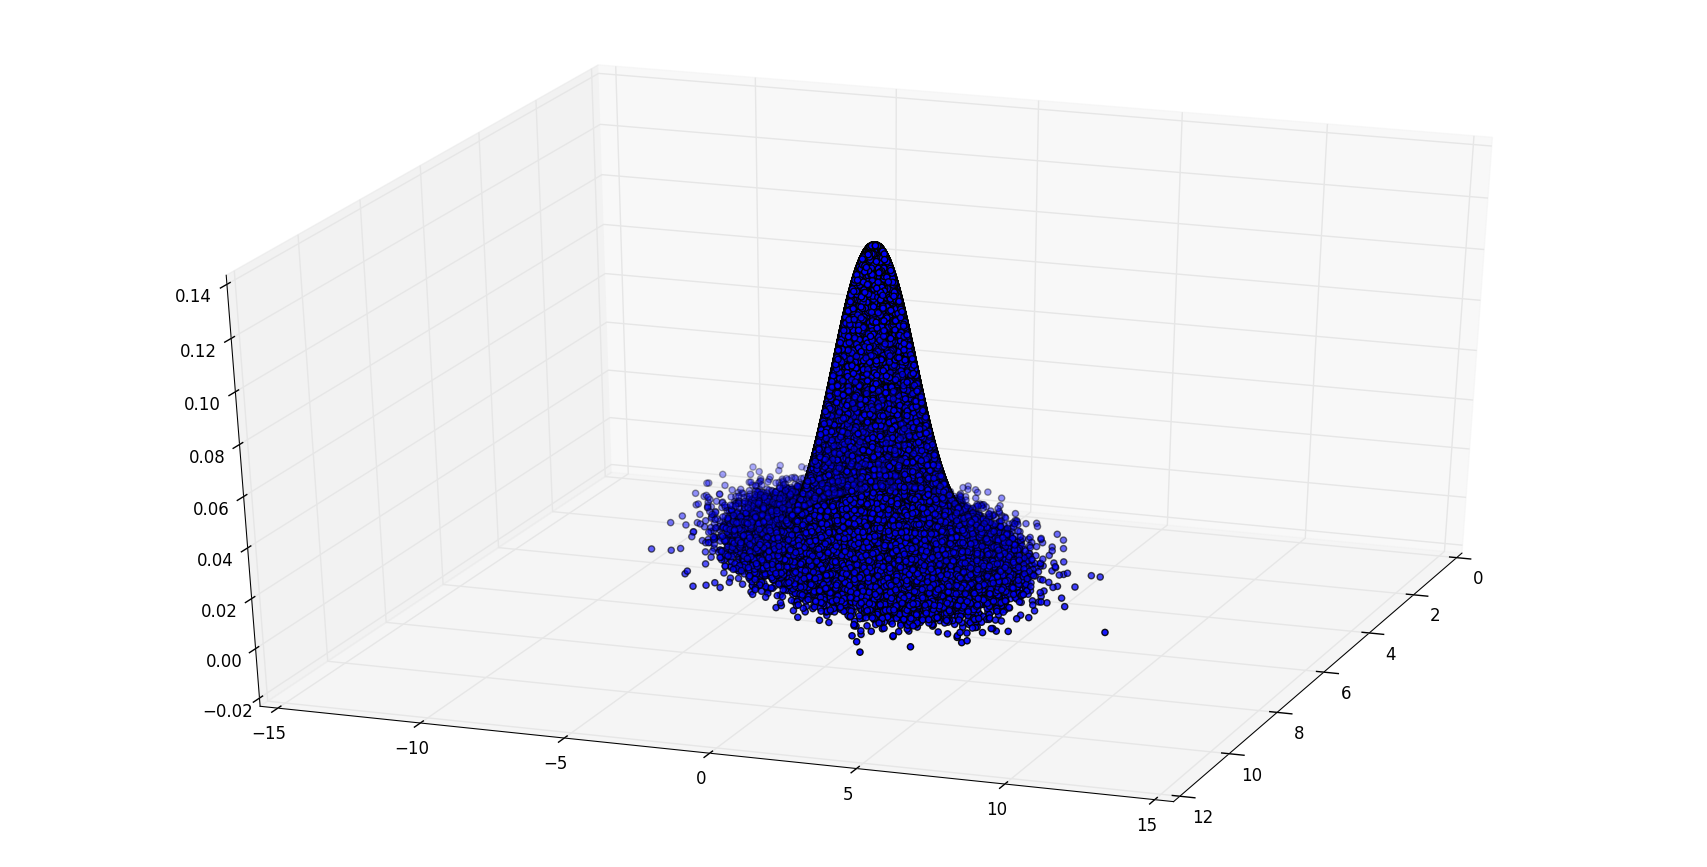
\includegraphics[width=1.0\linewidth]{figure/gibbs2}
	\caption{利用Gibbs采样法产生的二维Gauss分布}
	\label{fig:gibbs2}
	\end{figure}

%----------------------------------------------------------------------------------------
%	APPENDICES SECTION
%----------------------------------------------------------------------------------------

\newpage
\onecolumn
\begin{appendices}
\section{Box-Muller生成一维Gauss分布}
Here is the program by Box-Muller Method to generate 1 dimensional Gauss distribution in Python programming language.\\
\textbf{\textcolor[rgb]{0.98,0.00,0.00}{Input Python source:}}
\lstinputlisting[language=Python]{./program/Box-Muller.py}
\newpage
\section{Gibbs采样法生成二维Gauss分布}
Here is the program by Gibbs sampling Method to generate 2 dimensional Gauss distribution in Python programming language.\\
\textbf{\textcolor[rgb]{0.98,0.00,0.00}{Input Python source:}}
\lstinputlisting[language=Python]{./program/Gibbs.py}
\end{appendices}

%----------------------------------------------------------------------------------------
%	REFERENCE
%----------------------------------------------------------------------------------------

\newpage
\renewcommand\refname{参考文献}
\begin{thebibliography}{99}
\bibitem{ref1}G. E. P. Box and Mervin E. Muller, A Note on the Generation of Random Normal Deviates, The Annals of Mathematical Statistics (1958), Vol. 29, No. 2 pp. 610–611 doi:10.1214/aoms/1177706645, JSTOR 2237361.
\bibitem{ref2}Sheldon Ross, A First Course in Probability, (2002), pp. 279–281.
\bibitem{ref3}J. Bell: 'Algorithm 334: Normal random deviates', Communications of the ACM, vol. 11, No. 7. 1968.
\bibitem{ref4}R. Knopp: 'Remark on algorithm 334 [G5]: normal random deviates', Communications of the ACM, vol. 12, No. 5. 1969.
\bibitem{ref5}Everett F. Carter, Jr., The Generation and Application of Random Numbers, Forth Dimensions (1994), Vol. 16, No. 1 \& 2.
\bibitem{ref6}Note that the evaluation of $2\pi U_{1}$ is counted as one multiplication because the value of $2\pi$ can be computed in advance and used repeatedly.
\bibitem{ref7}Link, William A.; Eaton, Mitchell J. (2012-02-01). "On thinning of chains in MCMC". Methods in Ecology and Evolution. 3 (1): 112–115. doi:10.1111/j.2041-210X.2011.00131.x. ISSN 2041-210X.
\bibitem{ref8}Geman, S.; Geman, D. (1984). "Stochastic Relaxation, Gibbs Distributions, and the Bayesian Restoration of Images". IEEE Transactions on Pattern Analysis and Machine Intelligence. 6 (6): 721–741. doi:10.1109/TPAMI.1984.4767596.
\bibitem{ref9}Gilks, W. R.; Best, N. G.; Tan, K. K. C. (1995-01-01). "Adaptive Rejection Metropolis Sampling within Gibbs Sampling". Journal of the Royal Statistical Society. Series C (Applied Statistics). 44 (4): 455–472. JSTOR 2986138.
\bibitem{ref10}Meyer, Renate; Cai, Bo; Perron, François (2008-03-15). "Adaptive rejection Metropolis sampling using Lagrange interpolation polynomials of degree 2". Computational Statistics \& Data Analysis. 52 (7): 3408–3423. doi:10.1016/j.csda.2008.01.005.
\bibitem{ref11}Martino, L.; Read, J.; Luengo, D. (2015-06-01). "Independent Doubly Adaptive Rejection Metropolis Sampling Within Gibbs Sampling". IEEE Transactions on Signal Processing. 63 (12): 3123–3138. doi:10.1109/TSP.2015.2420537. ISSN 1053-587X.
\end{thebibliography} 

%----------------------------------------------------------------------------------------
\end{CJK*}
\end{document}
